\documentclass{beamer}

\usepackage{graphicx}
\usepackage{framed}

\begin{document}
	\begin{frame}
		\vspace{-0.5cm}
\begin{figure}
\centering
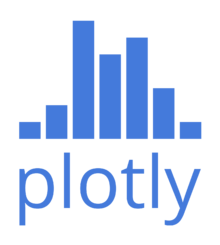
\includegraphics[width=0.55\linewidth]{plotlylogo}
\end{figure}

	\Large
\begin{itemize}
	\item \texttt{Kevin O'Brien} 
 \\ {\Large \texttt{(University of Limerick)}}
\end{itemize}	
	
\end{frame}
%============================================%
\begin{frame}
	\frametitle{plotly}
	\large		
	\begin{figure}
		\centering
		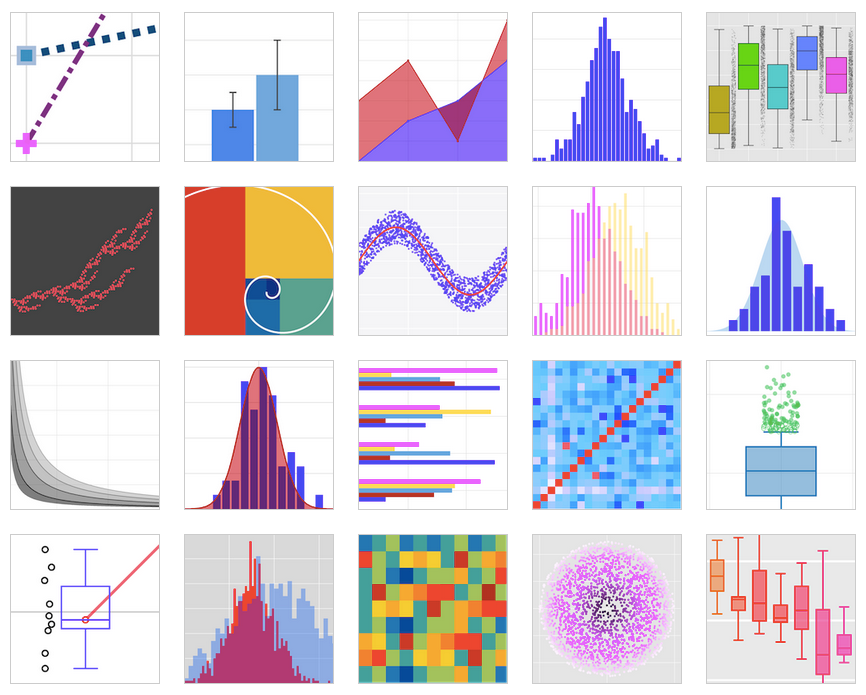
\includegraphics[width=0.8\linewidth]{plotlygallery}
	\end{figure}
	
\end{frame}


%========================================%
\begin{frame}
	\Large
	\texttt{Kevin O'Brien}
	\medskip
	\begin{itemize}
		\item Background in Statistical Computing \\
		{\large (R, Python, Julia, SPSS, SAS)}
		\medskip
		\item Formerly taught undergraduate statistics and analytics courses at University of Limerick.
		\medskip
		\item Work with a lot of career-young professionals.
		\medskip
		\item F.Y.I. I have no connection to \texttt{plot.ly}
	\end{itemize}
\end{frame}


\begin{frame}
	\vspace{-0.5cm}
	\begin{figure}
		\centering
		
\includegraphics[width=1.05\linewidth]{plotlyindustry}
	\end{figure}
	Aerospace, Material Science, Energy Prospecting etc
\end{frame}
%============================================%
\begin{frame}
\frametitle{plotly}
\Large	
About \texttt{plot.ly}\\
\textit{ (from company site)}

\begin{framed}

\textit{plotly is the state of the art in data visualization, dashboards, and collaborative analysis, that can be used to make carts and dashboards.}
\end{framed}
\end{frame}
%=============================================%
\begin{frame}
\frametitle{plotly}
\Large
\begin{figure}
\centering
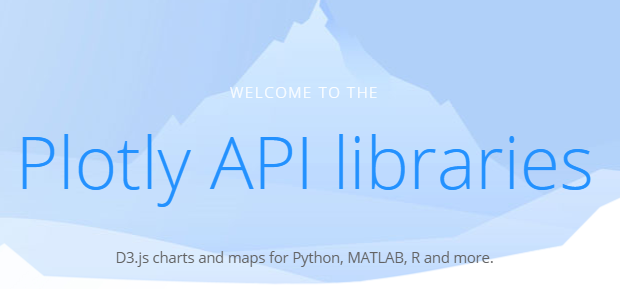
\includegraphics[width=1.05\linewidth]{plotlyapis1}
\end{figure}

\end{frame}
%==================================%
\begin{frame}
\frametitle{plotly}
\Large	
\begin{itemize}
	\item \texttt{plotly}'s graphing libraries makes interactive, publication-quality graphs online, with libraries for Python, R, MATLAB, Perl, Julia, Arduino, and REST.
\end{itemize}
\begin{figure}
\centering
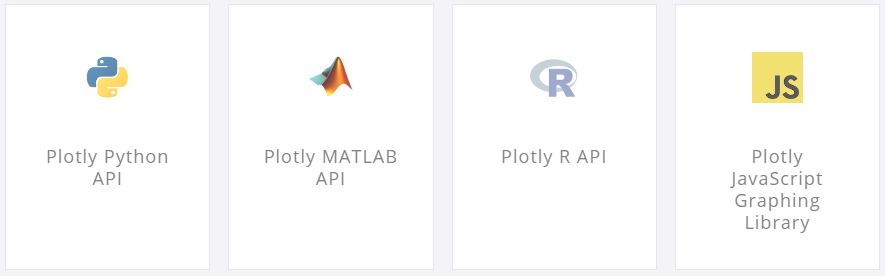
\includegraphics[width=1.05\linewidth]{plotlyapis}

\end{figure}

\end{frame}
%============================================%

\begin{frame}
\frametitle{plotly}
\Large	
	\texttt{Technology}
\begin{itemize}
	\item Plotly was built in Python and the Django framework, with a front end using JavaScript -- primarily the visualization library D3, HTML and CSS. 
	\item Files are hosted on Amazon S3. 
	\item Visualizations can't be viewed unless they're shared even if someone guesses the URL.
\end{itemize}
\end{frame}

%=============================================%
\begin{frame}[fragile]
	\Large
\vspace{-1cm}

	\begin{figure}
\centering
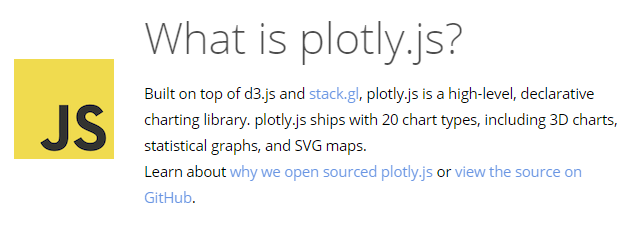
\includegraphics[width=1.10\linewidth]{plotlyjs}

\end{figure}
Built on top of \texttt{d3.js} and \texttt{stack.gl}, \texttt{plotly.js} is a high-level, declarative charting library.
{
\large
\begin{verbatim}
Source: http://plot.ly/javascript/
\end{verbatim}
}
\end{frame}

%=============================================%
\begin{frame}[fragile]
	\large
\texttt{Installation}
\begin{framed}
\begin{verbatim}
pip install plotly
\end{verbatim}
\end{framed}
	\begin{figure}
\centering
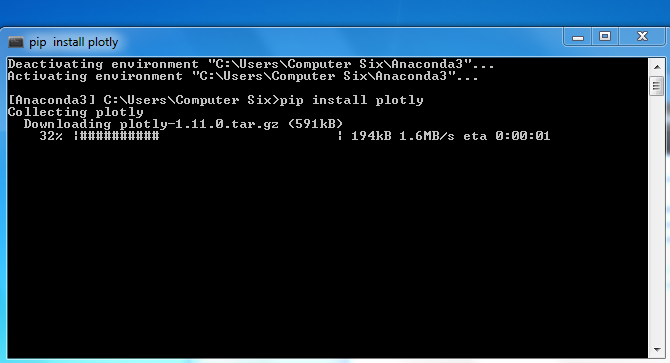
\includegraphics[width=0.95\linewidth]{pipinstallplotly}

\end{figure}
\end{frame}
%=============================================%
\begin{frame}
\begin{figure}
\centering

\includegraphics[width=0.9\linewidth]{github-logo}

\end{figure}
	
\end{frame}
%=============================================%
\begin{frame}
\large
\texttt{My plotLy Account}
\begin{figure}
\centering
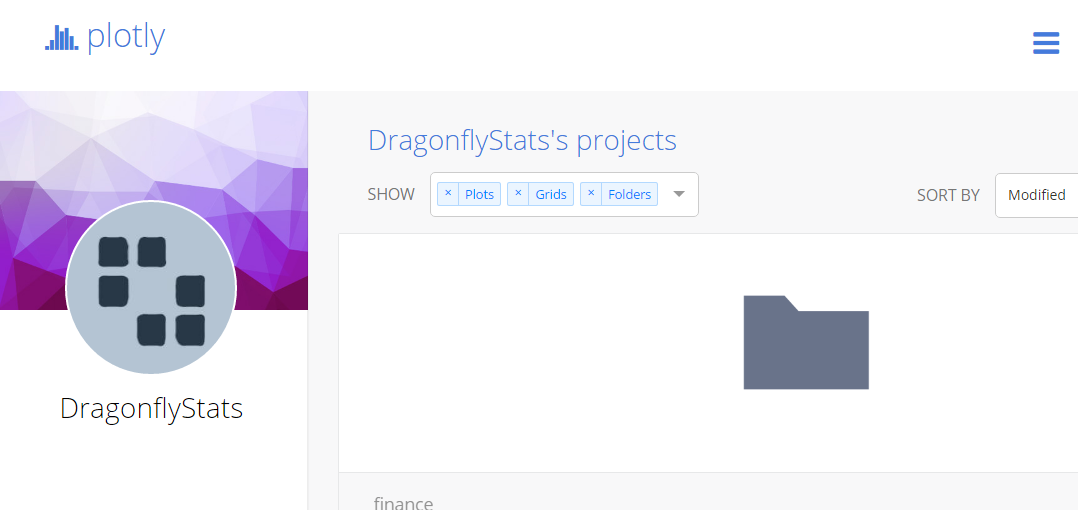
\includegraphics[width=01.1\linewidth]{plotlyprofile}
\end{figure}

\end{frame}

%===========================================================%
%=======================%
\begin{frame}[fragile]
	\Large
\texttt{Initialization for Online Plotting}\\
\textit{(from www.plot.ly)}
\medskip
\begin{itemize}
	\item \texttt{plotly} provides a web-service for hosting graphs! \medskip
	\item Create a free account to get started. 
	\medskip
	\item Graphs are saved inside your online \texttt{plotly} account and you control the privacy. 

\end{itemize}

\end{frame}
%===========================================================%

%=======================%
\begin{frame}[fragile]
\frametitle{plotly}
	\Large
	\texttt{Accessing Your Account}
	\begin{framed}
		\begin{verbatim}
		
		import plotly 
		
		plotly.tools.set_credentials_file(
				username='DemoAccount', 
				api_key='lr1c37zw81')
		
		\end{verbatim}
	\end{framed}
	Find your API key on your account page.
\end{frame}
%====================================================%
%=========================================================%
\begin{frame}
	\frametitle{plotly}
\Large
\texttt{\texttt{plot()} and \texttt{iplot() }}
\medskip
\begin{itemize}
	\item When plotting online, the plot and data will be saved to your plotly account.  \smallskip
	\item There are two methods for plotting online: \texttt{py.plot()} and \texttt{py.iplot()}. \\ Both options create a unique url for the plot and save it in your plotly account. \smallskip
	\item Use \texttt{py.plot()} to return the unique url and optionally open the url. \smallskip
	\item Use \texttt{py.iplot()} when working in a Jupyter Notebook to display the plot in the notebook.
\end{itemize}
\end{frame}
%=========================================================%
%====================================================%
\begin{frame}
	\large
	\texttt{OHLC chart}
\begin{itemize}
	\item 	OHLC or open-high-low-close chart is a type of chart used to illustrate how the price of a stock or bond changed over time. 
	
	\item Vertical line on the chart shows the price range (the highest and lowest prices).
\end{itemize}	

\end{frame}
%=======================================%

%======================================%
%https://plot.ly/~shikibm/77.png

\end{document}
